%==================================================================================================
\chapter{Formulação numérica para dinâmica não linear dos sólidos} \label{EGDS}
%==================================================================================================

Em se tratando de sólidos de comportamento hiperelástico, dada à natureza da lei constitutiva e à adequação da descrição Lagrangiana, é conveniente o uso de abordagens energéticas de modo a obter o equacionamento em forma fraca, seguido da aplicação da técnica de elementos finitos e de processos para solução numérica do sistema resultante. Para tal, deve-se primeiramente definir o conceito de energia total ($\Pi$) de um sistema, que pode ser entendido como a soma de todas as parcelas de energia relevantes ao problema. Nos casos mais comuns, tem-se uma parcela de energia potencial das forças externas atuantes no corpo ($\mathbb{P}$), uma parcela de energia de deformação elástica ($\mathbb{U}$) e parcela de energia cinética ($\mathbb{K}$). Dessa forma, o funcional de energia total é dado por:

\begin{equation}
    \Pi=\mathbb{P}+\mathbb{U}+\mathbb{K}\text{.}
    \label{FuncionalEnergia}
\end{equation}

Busca-se encontrar a configuração de equilíbrio do sólido, e para tal, a conservação da energia deve ser respeitada. Dessa forma postula-se o primeiro teorema variacional, que aponta que, para se obter o equilíbrio em um sólido sujeito a forças externas conservativas, a primeira variação da energia total deve ser nula para qualquer variação admissível nas incógnitas do problema, ou seja:

\begin{equation}
    \delta^{(1)}\Pi=0\forall\delta\BB{u}|\delta\BB{u}=\BB{0}\text{ em }\Gamma_D\text{,}
\end{equation}

\noindent em que $\Gamma_D$ é a parcela da fronteira onde os deslocamentos são prescritos. Já o segundo teorema trata-se da estabilidade desse equilíbrio, onde para se atingir o equilíbrio estável a segunda variação da energia total deve ser positiva para qualquer variação admissível, ou seja:

\begin{equation}
    \delta^{(2)}\Pi>0\forall\delta\BB{u}|\delta\BB{u}=\BB{0}\text{ em }\Gamma_D\text{.}
\end{equation}

Sendo assim, primeiramente procura-se anular a primeira variação da energia total:

\begin{equation}
    \delta\Pi=\delta\mathbb{P}+\delta\mathbb{U}+\delta\mathbb{K}=0\text{,}
\end{equation}

\noindent o que leva à necessidade de se determinar a primeira variação de $\mathbb{U}$. Para isso, é necessária a consideração de um modelo constitutivo que permita, juntamente com as demais equações da cinemática do modelo estrutural, descrever a evolução da energia de deformação em função das variáveis principais do problema. Um possível modelo constitutivo é o de Saint-Venant-Kirchhoff, dado por:

\begin{equation}
    u_e^{SVK}=\frac{S_{ij}\mathbb{E}_{ij}}{2}\text{,}
\end{equation}

\noindent no qual $\mathbb{E}_{ij}$ é a medida de deformação de Green-Lagrange, sendo bem definida no Apêndice \ref{Ap:CSD}, e $S_{ij}$ é o tensor de Piola-Kirchhoff de segunda espécie, que pode ser determinado como:

\begin{equation}
    S_{ij}=\script{C}_{ijkl}\mathbb{E}_{kl}\text{,}
    \label{eq:CSD-S}
\end{equation}

\noindent sendo $\script{C}_{ijkl}$ o tensor constitutivo de quarta ordem:

\begin{equation}
    \script{C}_{ijkl}=2G\delta_{ik}\delta_{jl}+\frac{2G\nu}{1-2\nu}\delta_{ij}\delta_{kl}
\end{equation}

\noindent no qual $\nu$ é o coeficiente de Poisson e $G$ é o módulo de elasticidade transversal, dado em função do módulo de elasticidade longitudinal (ou Módulo de Young) $E$ como:

\begin{equation}
    G=\frac{E}{2(1+\nu)}\text{.}
\end{equation}

Assim, as parcelas de energia ficam dadas por:

\begin{subequations}
    \begin{align}
         & \mathbb{U}=\frac{1}{2}\intDomi{S_{ij}\mathbb{E}_{ij}}\text{,}    \\
         & \mathbb{P}=-F_i^aY_i^a-\intFronti{t_iy_i^m}\text{ e}             \\
         & \mathbb{K}=\frac{1}{2}\intDomi{\rho_0\dot{y}_i\dot{y}_i}\text{,}
    \end{align}
\end{subequations}

\noindent onde $\Omega_0$ é o domínio de análise em sua configuração inicial, cuja fronteira é $\Gamma_0=\partial\Omega_0$, $F_i^a$ é uma força concentrada aplicada sobre um ponto $a$ na direção $i$, cuja posição atual é $Y_i^a$, $t_i$ é uma força distribuída sobre uma superfície média da casca ($y_i$) e $\rho_0$ é a massa específica inicial do contínuo.

%\noindent O Apêndice \ref{Ap:CSD} trata de forma mais detalhada o comportamento para casos multiaxiais.

%==================================================================================================
\section{Método dos Elementos Finitos Posicional Aplicado a Elementos de Casca} \label{MEFP}
%==================================================================================================

Os elementos de casca podem ser ser entendidos como aqueles em que uma de suas dimensões é muito menor que as demais. Assim, é possível tomar como referência a superfície média do elemento para mapear os pontos que o compõem, facilitando, assim, a computação desses elementos. Isso é feito a partir da consideração de vetores generalizados nas configurações inicial e atual, assim como também será inserido um termo adicional para evitar o travamento volumétrico.

A formulação que será apresentada a seguir segue a cinemática de Reissner-Mindlin e foi proposta por \citeonline{coda2007alternative}, sendo aplicada ao contexto da interação fluido-estrutura por \citeonline{sanches2011acoplamento,sanches2013unconstrained}.

O método de solução numérica partirá de uma abordagem energética, com discretização espacial feita a partir de funções de forma e a discretização temporal feita por meio de aproximação de Newmark, sendo o sistema algébrico resultante resolvido via método de Newton-Raphson.

%\textcolor{red}{Deixe a parcela dissipativa de fora...}

%==================================================================================================
\subsection{Cinemática de Reissner-Mindlin}
%==================================================================================================

Para se realizar o cálculo dessas propriedades, será considerada uma aproximação das variáveis por meio de polinômios aproximadores (funções de forma), na qual será utilizado um espaço intermediário de coordenadas paramétricas ($\BB{\xi}$) no procedimento. A Figura \ref{fig:Mapeamento} apresenta esquematicamente o mapeamento das coordenadas da superfície média em seus respectivos espaços.

\begin{figure}[h!]
    \centering
    \caption{Mudança de configuração.}
    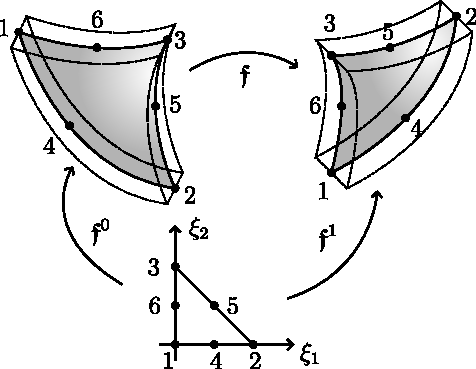
\includegraphics[width=.4\linewidth]{Figuras/Mapeamento.pdf}
    \\Fonte: Autoria Própria (\the\year).
    \label{fig:Mapeamento}
\end{figure}

Sendo assim, realiza-se o mapeamento dos pontos da superfície média do elemento, em suas configurações inicial ($x_i^m$) e atual ($y_i^m$), através da aproximação por funções de forma de elementos planos:

\begin{subequations}
    \begin{align}
         & f_i^{m0}=x_i^m=X_i^aN_a(\xi_1,\xi_2)\text{,} \\
         & f_i^{m1}=y_i^m=Y_i^aN_a(\xi_1,\xi_2)\text{,}
    \end{align}
\end{subequations}

\noindent em que $f_i^{m0}$ e $f_i^{m1}$ são as funções de mudança de configuração da superfície média $\Omega_\xi\to\Omega_0$ e $\Omega_\xi\to\Omega$, respectivamente, onde $\Omega_\xi$ é o espaço paramétrico e $\Omega$ é a configuração atual do contínuo, $X_i^a$ e $Y_i^a$ são as coordenadas do nó $a$, pertencente à superfície média, nas configurações inicial e atual, respectivamente, e $N_a(\xi_1,\xi_2)$ o valor da função de forma associada à esse nó.

Já os demais pontos do elemento podem ser mapeados por meio de um vetor generalizado como:

\begin{subequations}
    \begin{align}
         & f_i^0=x_i^m+v_i^0\text{,} \\
         & f_i^1=y_i^m+v_i^1\text{,}
    \end{align}
\end{subequations}

\noindent que na configuração inicial é denotado por $v_i^0$, o qual é normal unitário à superfície média inicial, e e $v_i^1$, que não é unitário nem normal à superfície média. Em uma discretização por elementos finitos esses vetores podem ser dados por:

\begin{subequations}
    \begin{align}
         & v_i^0=\frac{h_0}{2}N_ a(\xi_1,\xi_2)(V^0)_i^a\xi_3\text{,}                              \\
         & v_i^1=\frac{h_0}{2}N_ a(\xi_1,\xi_2)(V^1)_i^a[\xi_3+\alpha(\xi_1,\xi_2)\xi_3^2]\text{,}
    \end{align}
\end{subequations}

\noindent sendo $h_0$ a espessura inicial da casca, $(V^0)_i^a$ e $(V^1)_i^a$ os valores dos vetores generalizados na configuração inicial e atual sobre o nó $a$, respectivamente, e $\alpha(\xi_1,\xi_2)$ é um enriquecimento nodal inserido ao problema com a finalidade de evitar travamento volumétrico, o qual pode ser entendido como a taxa de variação linear da deformação, que é aproximada por função de forma como:

\begin{equation}
    \alpha(\xi_1,\xi_2)=\Alpha^aN_a(\xi_1,\xi_2)\text{,}
\end{equation}

\noindent sendo $\Alpha^a$ seu valor sobre o nó $a$ \cite{sanches2013unconstrained,sanches2014fluid}.

Sendo assim, o problema possui como graus de liberdade as posições nodais atuais ($Y_i^a$), os valores do vetor generalizado na configuração atual ($(V^1)_i^a$) e a taxa de variação linear da deformação ($\Alpha^a$).

%Além disso, note que $\BB{f}(\BB{x},t)=\BB{f}^1((\BB{f}^0)^{-1},t)$, portanto é possível se obter o gradiente da função de mudança de configuração ($\BB{A}=\partial\BB{f}/\partial\BB{x}$) como $\BB{A}=\BB{A}^1\cdot(\BB{A}^0)^{-1}$, em que $A^0_{ij}=f^0_{i,j}$ e $A^1_{ij}=f^1_{i,j}$.

Assim, considera-se o princípio da conservação da energia como:

\begin{equation}
    \delta\Pi=\der{\Pi_0}{g_i}\delta g_i=0\text{,}
\end{equation}

\noindent em que $\BB{g}$ representa o vetor que contém todos os graus de liberdade do problema.

Logo, precisa-se calcular a derivada de $\Pi_0$ em relação à $Y_i^a$, $({V}^1)_i^a$ e $\Alpha^a$. Dessa forma tem-se as seguintes derivadas:

\begin{subequations}
    \begin{equation}
        \der{\Pi_0}{Y_i^a}=\der{\mathbb{U}}{Y_i^a}+\intDomi{\rho_0N_a\ddot{y}_i}-F_i^a-\intFronti{N_at_i}=0\text{,}
    \end{equation}
    \begin{equation}
        \der{\Pi_0}{(V^1)_i^a}=\der{\mathbb{U}}{(V^1)_i^a}+\intDomi{\rho_0\frac{h_0}{2}N_a(\xi_3+\alpha\xi_3^2)\ddot{y}_i}=0\text{,}
    \end{equation}
    \begin{equation}
        \der{\Pi_0}{\Alpha^a}=\der{\mathbb{U}}{\Alpha^a}+\intDomi{\rho_0\frac{h_0}{2}N_aN_b(V^1)_i^b\xi_3^2\ddot{y}_i}=0\text{,}
    \end{equation}
\end{subequations}

\noindent sendo possível definir um vetor resíduo $\BB{r}$ como:

\begin{equation}
    r_i^a(\BB{Y},\BB{V}^1,\BB{\Alpha})=(F^\mathrm{int})_i^a+(F^\mathrm{inerc})_i^a-(F^\mathrm{c})_i^a=0\text{,}
    \label{eq:CSD-g}
\end{equation}

\noindent sendo $\BB{Y}$, $\BB{V}^1$ e $\BB{\Alpha}$ os vetores dos graus de liberdade nodais do elemento analisado:

\begin{subequations}
    \begin{align}
         & (F^\mathrm{int})_i^a=\intDomi{\der{u_e}{g_i^a}}=\intDomi{S_{kl}\der{\mathbb{E}_{kl}}{g_i^a}}\text{,}\label{eq:CSD-Fint} &  & \text{Forças internas}      \\
         & (F^\mathrm{inerc})_i^a=\intDomi{\rho_0\der{y_j}{g_i^a}\ddot{y}_j}\text{,}\label{eq:CSD-Finerc}                          &  & \text{Forças inerciais}     \\
         & (F^\mathrm{c})_i^a=F_j^b\der{Y_j^b}{g_i^a}+\intFronti{t_j\der{y_j^m}{g_i^a}}\text{ e}\label{eq:CSD-Fc}                  &  & \text{Forças conservativas}
    \end{align}
    \label{eq:CSD-F}
\end{subequations}

Portanto o problema ser resolvido é descrito como: determinar $\BB{Y}$, $\BB{V}^1$ e $\BB{\Alpha}$ tais que $\BB{r}(\BB{Y},\BB{V}^1,\BB{\Alpha})=\BB{0}$.

Como é possível perceber, o cálculo de $\BB{r}$ é dependente não somente dos graus de liberdade, mas também das derivadas temporais de primeira e segunda ordem das posições. Sendo assim, se faz necessária a consideração de um integrador temporal, o qual será utilizado o integrador temporal de Newmark, devido à capacidade de respeitar a conservação de momento linear para $\gamma=1/2$ e apresentando bons resultados para modelagem de elementos de casca, conforme apresentado por \citeonline{sanches2013unconstrained}.

A aproximação realizada pelo integrador de Newmark é dada por:

\begin{subequations}
    \begin{equation}
        g_i^{n+1}=g_i^n+\dot{g}_i^n\Delta t+\Delta t^2\bigpar{\bigpar{\frac{1}{2}-\beta}\ddot{g}_i^n+\beta\ddot{g}_i^{n+1}}\text{ e}
    \end{equation}
    \begin{equation}
        \dot{g}_i^{n+1}=\dot{g}_i^n+\Delta t(1-\gamma)\ddot{g}_i^n+\gamma\ddot{g}_i^{n+1}\Delta t\text{,}
    \end{equation}
\end{subequations}

\noindent sendo o superíndice $n$ e $n+1$ a indicação do passo de tempo analisado ($t_n$ e $t_{n+1}$), $\Delta t$ o intervalo de tempo discretizado e $\beta$ e $\gamma$ parâmetros livres, que devem ser escolhidos de forma a garantir a convergência do método, sendo arbitrados valores de $\beta=1/4$ e $\gamma=1/2$, garantindo a estabilidade incondicional do método \cite{LINDFIELD2019239}.

Isolando-se os termos incógnitos em função de variáveis não derivadas no tempo em $n+1$ e daquelas já conhecidas tem-se:

\begin{subequations}
    \begin{equation}
        \ddot{g}_i^{n+1}=\frac{g_i^{n+1}-g_i^n}{\beta\Delta t^2}-\frac{\dot{g}_i^n}{\beta\Delta t}+\bigpar{1-\frac{1}{2\beta}}\ddot{g}_i^n
    \end{equation}
    \begin{equation}
        \dot{g}_i^{n+1}=\frac{\gamma}{\beta\Delta t}(g_i^{n+1}-g_i^n)+\bigpar{1-\frac{\gamma}{\beta}}\dot{g}_i^n+\Delta t\bigpar{1-\frac{\gamma}{2\beta}}\ddot{g}_i^n\text{.}
    \end{equation}
    \label{eq:CSD-Newmark2}
\end{subequations}

Já para procurar valores de $\BB{g}$ que anulem $\BB{r}$, utiliza-se o Método de Newton-Raphson, o qual parte da aproximação por série de Taylor truncada no termo de primeira ordem:

\begin{equation}
    \begin{split}
        &\BB{r}(\BB{g}+\Delta\BB{g})=\BB{r}(\BB{g})+\apderp{\BB{r}}{\BB{g}}{\BB{g}}\Delta\BB{g}=\\
        &\BB{r}(\BB{Y},\BB{V}^1,\BB{\Alpha})+\apderp{\BB{r}}{\BB{Y}}{\BB{Y}}\Delta\BB{Y}+\apderp{\BB{r}}{\BB{V}^1}{\BB{V}^1}\Delta\BB{V}^1+\apderp{\BB{r}}{\BB{\Alpha}}{\BB{\Alpha}}\Delta\BB{\Alpha}=\BB{0}\text{.}
    \end{split}
\end{equation}

\noindent Dessa forma, necessita-se do cálculo de uma matriz Hessiana ($H_{ij}^{ab}$):

\begin{equation}
    H_{ij}^{ab}=\frac{\partial^2\Pi_0}{\partial g_j^b\partial g_i^a}=\der{r_i^a}{g_j^b}\text{.}
\end{equation}

Substituindo-se as derivadas temporais da aproximação de Newmark em $\BB{r}$ e realizando as devidas simplificações, obtém-se:

\begin{equation}
    H_{ij}^{ab}=(H^\text{est})_{ij}^{ab}+\frac{M_{ij}^{ab}}{\beta\Delta t^2}+\intDom{\rho_0\ddot{y}_k\Dder{y_k}{g_j^b}{g_i^a}}\text{,}
    \label{eq:CSD-Hijab}
\end{equation}

\noindent sendo $(H^\text{est})_{ij}^{ab}$ a matriz hessiana estática elementar, $M_{ij}^{ab}$ a matriz de massa e $C_{ij}^{ab}$ a matriz de amortecimento, dadas por:

\begin{subequations}
    \begin{align}
         & (H^\text{est})_{ij}^{ab}=\Dder{\mathbb{U}}{g_j^b}{g_i^a}=\intDomi{\bigpar{\der{S_{kl}}{g_j^b}\der{\mathbb{E}_{kl}}{g_i^a}+S_{kl}\Dder{\mathbb{E}_{kl}}{g_i^a}{g_j^b}}}\text{ e} \\
         & M_{ij}^{ab}=\intDomi{\rho_0\der{y_k}{g_i^a}\der{y_k}{g_j^b}}\text{.}
    \end{align}
    \label{eq:CSD-HMC}
\end{subequations}

\noindent também observa-se que a derivada mista de $y_k$ em relação a $g_i^a$ e $g_j^b$ possuirá valores não-nulos apenas quando for derivada de forma cruzada em relação a $V^1$ e $\Alpha$.

Com isso, encontra-se um vetor de correções dos graus de liberdade ($\Delta\BB{g}$) como a solução do sistema:

\begin{equation}
    H_{ij}\Delta g_j=-r_i\text{,}
\end{equation}

\noindent tendo como critério de parada a medida do erro:

\begin{equation}
    \frac{\norm{\Delta\BB{Y}}}{\norm{\BB{X}}}\leq\text{tol,}
    \label{eq:CSD-erro}
\end{equation}

\noindent em que $\BB{X}$ o vetor de posições nodais iniciais e tol uma tolerância admitida.

%%==================================================================================================
%\subsection{Procedimento Computacional} \label{MEFP-Comp}
%%==================================================================================================
%
%Para a implementação computacional realizou-se uma integração em $\Omega_0$ e $\Gamma_0$ segundo a quadratura de hammer \cite{hammer1956numerical}, sendo a malha gerada %automaticamente via comunicação direta do algoritmo com o \textit{Gmsh} e o procedimento paralelizado utilizando o protocolo MPI presente na biblioteca PETSc. Demais informações %relevantes à implementação computacional são descritas detalhadamente no capítulo \ref{MetodologiaCronograma}.
%
%O algoritmo visto no Apêndice \ref{Ap:Shell-alg} apresentado na forma de pseudocódigo exemplifica o código implementado.

%==================================================================================================
\subsection{Exemplos de Verificação} \label{MEFP-Ex}
%==================================================================================================

Para verificação do código implementado, estudou-se para problemas estáticos: a simulação de \textit{Scordelis-Lo roof} e o problema de cilindro biengastado, enquanto para problemas dinâmicos estudou-se o comportamento de vigas engastadas. Tais simulações executadas, contendo os parâmetros de entrada, assim como a discretização de cada problema e os resultados obtidos, são apresentados nos Apêndices \ref{Ap:SLR}, \ref{Ap:Shell-cyl} e \ref{Ap:DinBeam}, para os respectivos problemas.